% vim: set spell spelllang=es syntax=tex :

\section{OpenMP: Open Multi-Prossesing}

\emph{OpenMP} es una API de bibliotecas y directivas al compilador para la
definición de paralelismo de alto nivel para sistemas de memoria compartida en
\emph{C}, \emph{C++} y \emph{Fortran} \cite{ompWeb}. La ventaja de \emph{OpenMP}
es que permite la creación de regiones paralelas, secciones criticas, tareas y
puntos de sincronización, simplemente marcando un bloque de código con unas
pocas directivas al compilador. \emph{OpenMP} originalmente implementaba solo el
modelo de \emph{fork and join}, pero a partir de la versión $3.0$ se agrego el
modelo de tareas explicitas \cite{openmp08}. Ambos modelos fueron utilizados para
la implementación del sistema.

El modelo de \emph{fork and join} fue propuesto por primera vez en
\cite{conway1963}. En este modelo, la ejecución del programa se ejecuta con un
solo hilo al comienzo de se ejecución y durante sus secciones secuenciales, al
hilo inicial se lo llama hilo principal. Cuando se encuentra una región de
trabajo compartido (o \emph{worksharing region}) de $N$ tareas, el hilo
principal crea $N-1$ nuevos hilos. Cada hilo (incluido el hilo principal)
ejecuta una de las $N$ tareas. Esta etapa es llamada \emph{fork}. El hilo
principal no continua la ejecución secuencial hasta que no han finalizado todas
las tareas paralelas. A esta sincronización se la llama \emph{join}. La figura
\ref{conway} muestra un ejemplo en el cual se crean dos tareas paralelas. El
modelo de \emph{fork and join} puede aplicarse tanto para paralelismo de tareas
como de datos. 

\begin{figure}[!h]

	\centering

	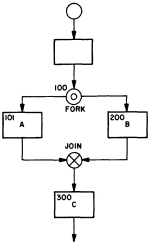
\includegraphics[height=0.25\textheight]{img/conway.pdf}

	\caption{Descripción original del modelo de \emph{fork and join}
	presentado por Melvin Conway en 1963 \cite{conway1963}.}

	\label{conway}

\end{figure}

Dado que la creación de hilos suele ser una operación costosa, la mayoría de las
implementaciones de \emph{OpenMP} suelen no destruir los hilos creados durante
el \emph{fork}, sino que se mantienen inactivos para ser reutilizados cuando se
encuentre otra región de trabajo compartido.

El segundo modelo implementado en \emph{OpenMP} a partir de la versión $3.0$ es
el de tareas. En este modelo cuando se encuentra una región de trabajo
compartido, se crea un conjunto de $N$ hilos de ejecución pero no se crean
tareas para esos hilos inmediatamente. Durante le ejecución de la región de
trabajo compartido, se crean tareas que son colocadas en una cola de ejecución.
Cuando un hilo de ejecución del conjunto esta libre se le asigna una tarea de la
cola de ejecución. Cuando un hilo termina de ejecutar una tarea, toma otra de la
cola de tareas o espera. Solo se destruyen los hilos cuando se termina la
ejecución de todas las tareas y se sale de la región de trabajo compartido.

Dado que la creación de las tareas se puede hacer luego de la creación de los
hilos de ejecución, este modelo permite una mayor distribución temporal de las
tareas creadas en una región compartida. También permite que una tarea cree
nuevas tareas dentro de la misma región.

\subsubsection{Directivas de OpenMP}

El control de la creación de hilos y tareas en \emph{OpenMP} se realiza a través
de directivas al compilador, en esta sección mencionaremos aquellas utilizadas
por el sistema propuesto. En \emph{C} y \emph{C++} todas las directivas toman la
forma de \textbf{\#pragma omp DIRECTIVA [OPCIONES]}.

La directiva más utilizada es \emph{parallel [num\_threads(N)]}, esta define una
región de trabajo paralelo y creando $N$ hilos de ejecución (si no se incluye
\emph{num\_threads(N)}, la cantidad de hilos se establece por medio de una
variable global, y en caso de que esta no este definida, dependerá de la
implementación). Cada hilo ejecutarán una tarea definida por el bloque inmediato
a la directiva, implementando el modelo \emph{fork and join}.

Si se desea que un bloque sea ejecutado solo por un hilo se pueden utilizar las
directivas \emph{single} y \emph{master}. Estas aseguraran que el bloque
inmediato sea ejecutado solo por uno de los hilos del grupo. En el caso de la
directiva \emph{single}, cualquiera de los hilos del grupo podrá ser elegido
para ejecutar el bloque, mientras que en el caso de \emph{master}, solo el
hilo principal del grupo lo ejecutarán.

Si se desea que cada hilo ejecute una tarea con código distinto se debe utilizar
la directiva \emph{parallel sections num\_threads(N)}. El bloque inmediato debe
contener a su vez bloques precedidos por la directiva \emph{section}. Al igual
que \emph{parallel}, esta directiva define una región de trabajo paralelo de $N$
hilos, pero el código de cada tarea esta definido por los bloques inmediatos a
las directivas \emph{section}. En caso de que se creen más hilos que las tareas
definidas, los hilos sobrantes no ejecutarán. El modelo implementado por esta
directiva es \emph{fork and join}.

Para la creación de una región de trabajo compartido bajo el modelo de tareas, se
utiliza la directiva \emph{parallel num\_threads(N)} para crear los $N$ hilos de
ejecución, seguida de la directiva \emph{master} para que solo el hilo principal
ejecute la tarea que crea las primeras tareas de la región de trabajo
compartido. Para la creación de cada tarea se debe utilizar la directiva
\emph{task} seguida del bloque que contiene el código a ejecutar por la tarea.

Si un hilo necesita esperar la finalización de las tareas que creo, antes de
continuar su ejecución, puede utilizar la directiva \emph{taskwait}.

Para definir secciones criticas se pueden utilizar las directivas \emph{critical
[NOMBRE]} y \emph{atomic}. La primera permite definir un bloque de complejidad
arbitraria como sección critica, e incluso permite definir bloques distintos
como la misma sección critica si comparten el mismo nombre. La segunda directiva
solo acepta bloques en los cuales se realiza una operación aritmética simple.

En la figura \ref{directivas} se muestra un código de ejemplo del uso de las
directivas presentadas junto con un diagrama mostrando una posible secuencia
de ejecución.

\begin{figure}[!h]

	\centering

	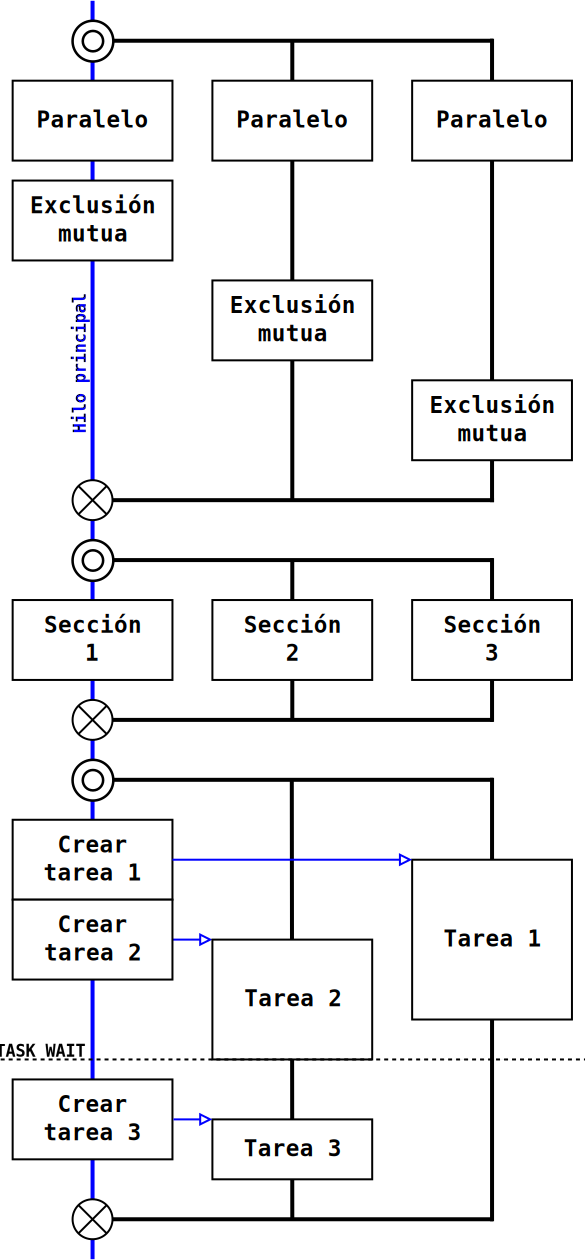
\includegraphics[height=0.40\textheight]{img/directivasOMP.pdf}
	\includegraphics{img/codigoDirectivasOMP.pdf}

	\caption{Código de ejemplo de uso de directivas de \emph{OpenMP} y
	posible secuencia de ejecución.}

	\label{directivas}

\end{figure}
